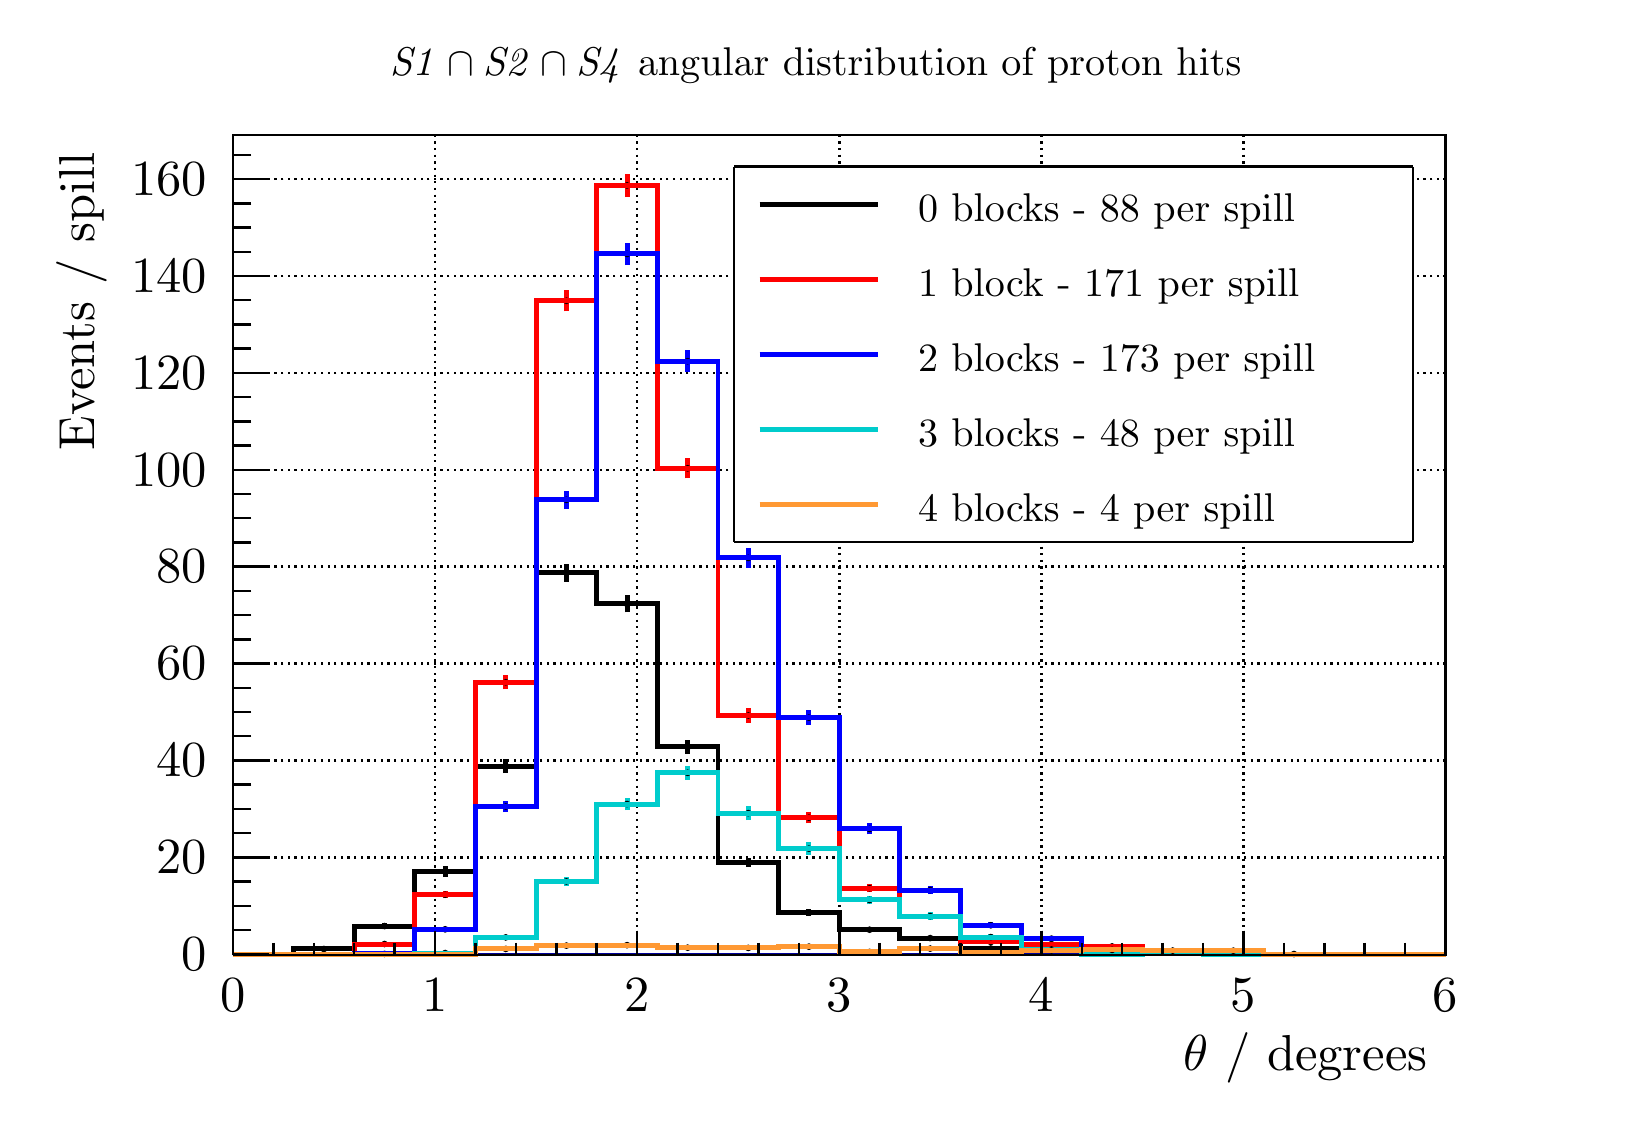
\begin{tikzpicture}
\pgfdeclareplotmark{cross} {
\pgfpathmoveto{\pgfpoint{-0.3\pgfplotmarksize}{\pgfplotmarksize}}
\pgfpathlineto{\pgfpoint{+0.3\pgfplotmarksize}{\pgfplotmarksize}}
\pgfpathlineto{\pgfpoint{+0.3\pgfplotmarksize}{0.3\pgfplotmarksize}}
\pgfpathlineto{\pgfpoint{+1\pgfplotmarksize}{0.3\pgfplotmarksize}}
\pgfpathlineto{\pgfpoint{+1\pgfplotmarksize}{-0.3\pgfplotmarksize}}
\pgfpathlineto{\pgfpoint{+0.3\pgfplotmarksize}{-0.3\pgfplotmarksize}}
\pgfpathlineto{\pgfpoint{+0.3\pgfplotmarksize}{-1.\pgfplotmarksize}}
\pgfpathlineto{\pgfpoint{-0.3\pgfplotmarksize}{-1.\pgfplotmarksize}}
\pgfpathlineto{\pgfpoint{-0.3\pgfplotmarksize}{-0.3\pgfplotmarksize}}
\pgfpathlineto{\pgfpoint{-1.\pgfplotmarksize}{-0.3\pgfplotmarksize}}
\pgfpathlineto{\pgfpoint{-1.\pgfplotmarksize}{0.3\pgfplotmarksize}}
\pgfpathlineto{\pgfpoint{-0.3\pgfplotmarksize}{0.3\pgfplotmarksize}}
\pgfpathclose
\pgfusepathqstroke
}
\pgfdeclareplotmark{cross*} {
\pgfpathmoveto{\pgfpoint{-0.3\pgfplotmarksize}{\pgfplotmarksize}}
\pgfpathlineto{\pgfpoint{+0.3\pgfplotmarksize}{\pgfplotmarksize}}
\pgfpathlineto{\pgfpoint{+0.3\pgfplotmarksize}{0.3\pgfplotmarksize}}
\pgfpathlineto{\pgfpoint{+1\pgfplotmarksize}{0.3\pgfplotmarksize}}
\pgfpathlineto{\pgfpoint{+1\pgfplotmarksize}{-0.3\pgfplotmarksize}}
\pgfpathlineto{\pgfpoint{+0.3\pgfplotmarksize}{-0.3\pgfplotmarksize}}
\pgfpathlineto{\pgfpoint{+0.3\pgfplotmarksize}{-1.\pgfplotmarksize}}
\pgfpathlineto{\pgfpoint{-0.3\pgfplotmarksize}{-1.\pgfplotmarksize}}
\pgfpathlineto{\pgfpoint{-0.3\pgfplotmarksize}{-0.3\pgfplotmarksize}}
\pgfpathlineto{\pgfpoint{-1.\pgfplotmarksize}{-0.3\pgfplotmarksize}}
\pgfpathlineto{\pgfpoint{-1.\pgfplotmarksize}{0.3\pgfplotmarksize}}
\pgfpathlineto{\pgfpoint{-0.3\pgfplotmarksize}{0.3\pgfplotmarksize}}
\pgfpathclose
\pgfusepathqfillstroke
}
\pgfdeclareplotmark{newstar} {
\pgfpathmoveto{\pgfqpoint{0pt}{\pgfplotmarksize}}
\pgfpathlineto{\pgfqpointpolar{44}{0.5\pgfplotmarksize}}
\pgfpathlineto{\pgfqpointpolar{18}{\pgfplotmarksize}}
\pgfpathlineto{\pgfqpointpolar{-20}{0.5\pgfplotmarksize}}
\pgfpathlineto{\pgfqpointpolar{-54}{\pgfplotmarksize}}
\pgfpathlineto{\pgfqpointpolar{-90}{0.5\pgfplotmarksize}}
\pgfpathlineto{\pgfqpointpolar{234}{\pgfplotmarksize}}
\pgfpathlineto{\pgfqpointpolar{198}{0.5\pgfplotmarksize}}
\pgfpathlineto{\pgfqpointpolar{162}{\pgfplotmarksize}}
\pgfpathlineto{\pgfqpointpolar{134}{0.5\pgfplotmarksize}}
\pgfpathclose
\pgfusepathqstroke
}
\pgfdeclareplotmark{newstar*} {
\pgfpathmoveto{\pgfqpoint{0pt}{\pgfplotmarksize}}
\pgfpathlineto{\pgfqpointpolar{44}{0.5\pgfplotmarksize}}
\pgfpathlineto{\pgfqpointpolar{18}{\pgfplotmarksize}}
\pgfpathlineto{\pgfqpointpolar{-20}{0.5\pgfplotmarksize}}
\pgfpathlineto{\pgfqpointpolar{-54}{\pgfplotmarksize}}
\pgfpathlineto{\pgfqpointpolar{-90}{0.5\pgfplotmarksize}}
\pgfpathlineto{\pgfqpointpolar{234}{\pgfplotmarksize}}
\pgfpathlineto{\pgfqpointpolar{198}{0.5\pgfplotmarksize}}
\pgfpathlineto{\pgfqpointpolar{162}{\pgfplotmarksize}}
\pgfpathlineto{\pgfqpointpolar{134}{0.5\pgfplotmarksize}}
\pgfpathclose
\pgfusepathqfillstroke
}
\definecolor{c}{rgb}{1,1,1};
\draw [color=c, fill=c] (0,0) rectangle (20,13.5319);
\draw [color=c, fill=c] (2.6,1.75915) rectangle (18,12.1787);
\definecolor{c}{rgb}{0,0,0};
\draw [c,line width=0.9] (2.6,1.75915) -- (2.6,12.1787) -- (18,12.1787) -- (18,1.75915) -- (2.6,1.75915);
\definecolor{c}{rgb}{1,1,1};
\draw [color=c, fill=c] (2.6,1.75915) rectangle (18,12.1787);
\definecolor{c}{rgb}{0,0,0};
\draw [c,line width=0.9] (2.6,1.75915) -- (2.6,12.1787) -- (18,12.1787) -- (18,1.75915) -- (2.6,1.75915);
\draw [c,line width=0.9] (2.6,1.75915) -- (18,1.75915);
\draw [c,dash pattern=on 0.80pt off 1.60pt ,line width=0.9] (2.6,12.1787) -- (2.6,1.75915);
\draw [c,dash pattern=on 0.80pt off 1.60pt ,line width=0.9] (5.16667,12.1787) -- (5.16667,1.75915);
\draw [c,dash pattern=on 0.80pt off 1.60pt ,line width=0.9] (7.73333,12.1787) -- (7.73333,1.75915);
\draw [c,dash pattern=on 0.80pt off 1.60pt ,line width=0.9] (10.3,12.1787) -- (10.3,1.75915);
\draw [c,dash pattern=on 0.80pt off 1.60pt ,line width=0.9] (12.8667,12.1787) -- (12.8667,1.75915);
\draw [c,dash pattern=on 0.80pt off 1.60pt ,line width=0.9] (15.4333,12.1787) -- (15.4333,1.75915);
\draw [c,dash pattern=on 0.80pt off 1.60pt ,line width=0.9] (18,12.1787) -- (18,1.75915);
\draw [c,line width=0.9] (2.6,1.75915) -- (2.6,12.1787);
\draw [c,dash pattern=on 0.80pt off 1.60pt ,line width=0.9] (18,1.77184) -- (2.6,1.77184);
\draw [c,dash pattern=on 0.80pt off 1.60pt ,line width=0.9] (18,3.00235) -- (2.6,3.00235);
\draw [c,dash pattern=on 0.80pt off 1.60pt ,line width=0.9] (18,4.23286) -- (2.6,4.23286);
\draw [c,dash pattern=on 0.80pt off 1.60pt ,line width=0.9] (18,5.46338) -- (2.6,5.46338);
\draw [c,dash pattern=on 0.80pt off 1.60pt ,line width=0.9] (18,6.69389) -- (2.6,6.69389);
\draw [c,dash pattern=on 0.80pt off 1.60pt ,line width=0.9] (18,7.9244) -- (2.6,7.9244);
\draw [c,dash pattern=on 0.80pt off 1.60pt ,line width=0.9] (18,9.15491) -- (2.6,9.15491);
\draw [c,dash pattern=on 0.80pt off 1.60pt ,line width=0.9] (18,10.3854) -- (2.6,10.3854);
\draw [c,dash pattern=on 0.80pt off 1.60pt ,line width=0.9] (18,11.6159) -- (2.6,11.6159);
\draw [c,dash pattern=on 0.80pt off 1.60pt ,line width=0.9] (18,1.77184) -- (2.6,1.77184);
\draw [c,dash pattern=on 0.80pt off 1.60pt ,line width=0.9] (18,11.6159) -- (2.6,11.6159);
\definecolor{c}{rgb}{0,0,0.6};
\draw [c,line width=0.9] (2.6,1.77184) -- (3.37,1.77184) -- (3.37,1.77184) -- (4.14,1.77184) -- (4.14,1.77184) -- (4.91,1.77184) -- (4.91,1.77184) -- (5.68,1.77184) -- (5.68,1.77184) -- (6.45,1.77184) -- (6.45,1.77184) -- (7.22,1.77184) --
 (7.22,1.77184) -- (7.99,1.77184) -- (7.99,1.77184) -- (8.76,1.77184) -- (8.76,1.77184) -- (9.53,1.77184) -- (9.53,1.77184) -- (10.3,1.77184) -- (10.3,1.77184) -- (11.07,1.77184) -- (11.07,1.77184) -- (11.84,1.77184) -- (11.84,1.77184) --
 (12.61,1.77184) -- (12.61,1.77184) -- (13.38,1.77184) -- (13.38,1.77184) -- (14.15,1.77184) -- (14.15,1.77184) -- (14.92,1.77184) -- (14.92,1.77184) -- (15.69,1.77184) -- (15.69,1.77184) -- (16.46,1.77184) -- (16.46,1.77184) -- (17.23,1.77184) --
 (17.23,1.77184) -- (18,1.77184);
\definecolor{c}{rgb}{0,0,0};
\draw [c,line width=0.9] (2.6,1.75915) -- (18,1.75915);
\draw [c,line width=0.9] (2.6,2.07174) -- (2.6,1.75915);
\draw [c,line width=0.9] (3.11333,1.91544) -- (3.11333,1.75915);
\draw [c,line width=0.9] (3.62667,1.91544) -- (3.62667,1.75915);
\draw [c,line width=0.9] (4.14,1.91544) -- (4.14,1.75915);
\draw [c,line width=0.9] (4.65333,1.91544) -- (4.65333,1.75915);
\draw [c,line width=0.9] (5.16667,2.07174) -- (5.16667,1.75915);
\draw [c,line width=0.9] (5.68,1.91544) -- (5.68,1.75915);
\draw [c,line width=0.9] (6.19333,1.91544) -- (6.19333,1.75915);
\draw [c,line width=0.9] (6.70667,1.91544) -- (6.70667,1.75915);
\draw [c,line width=0.9] (7.22,1.91544) -- (7.22,1.75915);
\draw [c,line width=0.9] (7.73333,2.07174) -- (7.73333,1.75915);
\draw [c,line width=0.9] (8.24667,1.91544) -- (8.24667,1.75915);
\draw [c,line width=0.9] (8.76,1.91544) -- (8.76,1.75915);
\draw [c,line width=0.9] (9.27333,1.91544) -- (9.27333,1.75915);
\draw [c,line width=0.9] (9.78667,1.91544) -- (9.78667,1.75915);
\draw [c,line width=0.9] (10.3,2.07174) -- (10.3,1.75915);
\draw [c,line width=0.9] (10.8133,1.91544) -- (10.8133,1.75915);
\draw [c,line width=0.9] (11.3267,1.91544) -- (11.3267,1.75915);
\draw [c,line width=0.9] (11.84,1.91544) -- (11.84,1.75915);
\draw [c,line width=0.9] (12.3533,1.91544) -- (12.3533,1.75915);
\draw [c,line width=0.9] (12.8667,2.07174) -- (12.8667,1.75915);
\draw [c,line width=0.9] (13.38,1.91544) -- (13.38,1.75915);
\draw [c,line width=0.9] (13.8933,1.91544) -- (13.8933,1.75915);
\draw [c,line width=0.9] (14.4067,1.91544) -- (14.4067,1.75915);
\draw [c,line width=0.9] (14.92,1.91544) -- (14.92,1.75915);
\draw [c,line width=0.9] (15.4333,2.07174) -- (15.4333,1.75915);
\draw [c,line width=0.9] (15.9467,1.91544) -- (15.9467,1.75915);
\draw [c,line width=0.9] (16.46,1.91544) -- (16.46,1.75915);
\draw [c,line width=0.9] (16.9733,1.91544) -- (16.9733,1.75915);
\draw [c,line width=0.9] (17.4867,1.91544) -- (17.4867,1.75915);
\draw [c,line width=0.9] (18,2.07174) -- (18,1.75915);
\draw [anchor=base] (2.6,1.04196) node[scale=1.82718, color=c, rotate=0]{0};
\draw [anchor=base] (5.16667,1.04196) node[scale=1.82718, color=c, rotate=0]{1};
\draw [anchor=base] (7.73333,1.04196) node[scale=1.82718, color=c, rotate=0]{2};
\draw [anchor=base] (10.3,1.04196) node[scale=1.82718, color=c, rotate=0]{3};
\draw [anchor=base] (12.8667,1.04196) node[scale=1.82718, color=c, rotate=0]{4};
\draw [anchor=base] (15.4333,1.04196) node[scale=1.82718, color=c, rotate=0]{5};
\draw [anchor=base] (18,1.04196) node[scale=1.82718, color=c, rotate=0]{6};
\draw [anchor= east] (18,0.460085) node[scale=1.82718, color=c, rotate=0]{$\theta$ / degrees};
\draw [c,line width=0.9] (2.6,1.75915) -- (2.6,12.1787);
\draw [c,line width=0.9] (3.062,1.77184) -- (2.6,1.77184);
\draw [c,line width=0.9] (2.831,2.07947) -- (2.6,2.07947);
\draw [c,line width=0.9] (2.831,2.3871) -- (2.6,2.3871);
\draw [c,line width=0.9] (2.831,2.69473) -- (2.6,2.69473);
\draw [c,line width=0.9] (3.062,3.00235) -- (2.6,3.00235);
\draw [c,line width=0.9] (2.831,3.30998) -- (2.6,3.30998);
\draw [c,line width=0.9] (2.831,3.61761) -- (2.6,3.61761);
\draw [c,line width=0.9] (2.831,3.92524) -- (2.6,3.92524);
\draw [c,line width=0.9] (3.062,4.23286) -- (2.6,4.23286);
\draw [c,line width=0.9] (2.831,4.54049) -- (2.6,4.54049);
\draw [c,line width=0.9] (2.831,4.84812) -- (2.6,4.84812);
\draw [c,line width=0.9] (2.831,5.15575) -- (2.6,5.15575);
\draw [c,line width=0.9] (3.062,5.46338) -- (2.6,5.46338);
\draw [c,line width=0.9] (2.831,5.771) -- (2.6,5.771);
\draw [c,line width=0.9] (2.831,6.07863) -- (2.6,6.07863);
\draw [c,line width=0.9] (2.831,6.38626) -- (2.6,6.38626);
\draw [c,line width=0.9] (3.062,6.69389) -- (2.6,6.69389);
\draw [c,line width=0.9] (2.831,7.00151) -- (2.6,7.00151);
\draw [c,line width=0.9] (2.831,7.30914) -- (2.6,7.30914);
\draw [c,line width=0.9] (2.831,7.61677) -- (2.6,7.61677);
\draw [c,line width=0.9] (3.062,7.9244) -- (2.6,7.9244);
\draw [c,line width=0.9] (2.831,8.23202) -- (2.6,8.23202);
\draw [c,line width=0.9] (2.831,8.53965) -- (2.6,8.53965);
\draw [c,line width=0.9] (2.831,8.84728) -- (2.6,8.84728);
\draw [c,line width=0.9] (3.062,9.15491) -- (2.6,9.15491);
\draw [c,line width=0.9] (2.831,9.46253) -- (2.6,9.46253);
\draw [c,line width=0.9] (2.831,9.77016) -- (2.6,9.77016);
\draw [c,line width=0.9] (2.831,10.0778) -- (2.6,10.0778);
\draw [c,line width=0.9] (3.062,10.3854) -- (2.6,10.3854);
\draw [c,line width=0.9] (2.831,10.693) -- (2.6,10.693);
\draw [c,line width=0.9] (2.831,11.0007) -- (2.6,11.0007);
\draw [c,line width=0.9] (2.831,11.3083) -- (2.6,11.3083);
\draw [c,line width=0.9] (3.062,11.6159) -- (2.6,11.6159);
\draw [c,line width=0.9] (3.062,1.77184) -- (2.6,1.77184);
\draw [c,line width=0.9] (3.062,11.6159) -- (2.6,11.6159);
\draw [c,line width=0.9] (2.831,11.9236) -- (2.6,11.9236);
\draw [anchor= east] (2.5,1.77184) node[scale=1.82718, color=c, rotate=0]{0};
\draw [anchor= east] (2.5,3.00235) node[scale=1.82718, color=c, rotate=0]{20};
\draw [anchor= east] (2.5,4.23286) node[scale=1.82718, color=c, rotate=0]{40};
\draw [anchor= east] (2.5,5.46338) node[scale=1.82718, color=c, rotate=0]{60};
\draw [anchor= east] (2.5,6.69389) node[scale=1.82718, color=c, rotate=0]{80};
\draw [anchor= east] (2.5,7.9244) node[scale=1.82718, color=c, rotate=0]{100};
\draw [anchor= east] (2.5,9.15491) node[scale=1.82718, color=c, rotate=0]{120};
\draw [anchor= east] (2.5,10.3854) node[scale=1.82718, color=c, rotate=0]{140};
\draw [anchor= east] (2.5,11.6159) node[scale=1.82718, color=c, rotate=0]{160};
\draw [anchor= east] (0.68,12.1787) node[scale=1.82718, color=c, rotate=90]{ Events / spill};
\draw [c,line width=1.8] (3.755,1.81789) -- (3.755,1.83839);
\draw [c,line width=1.8] (3.755,1.83839) -- (3.755,1.85888);
\foreach \P in {(3.755,1.83839)}{\draw[mark options={color=c,fill=c},mark size=2.402402pt,mark=*,mark size=1pt] plot coordinates {\P};}
\draw [c,line width=1.8] (4.525,2.08664) -- (4.525,2.12905);
\draw [c,line width=1.8] (4.525,2.12905) -- (4.525,2.17145);
\foreach \P in {(4.525,2.12905)}{\draw[mark options={color=c,fill=c},mark size=2.402402pt,mark=*,mark size=1pt] plot coordinates {\P};}
\draw [c,line width=1.8] (5.295,2.7576) -- (5.295,2.82384);
\draw [c,line width=1.8] (5.295,2.82384) -- (5.295,2.89009);
\foreach \P in {(5.295,2.82384)}{\draw[mark options={color=c,fill=c},mark size=2.402402pt,mark=*,mark size=1pt] plot coordinates {\P};}
\draw [c,line width=1.8] (6.065,4.07122) -- (6.065,4.16002);
\draw [c,line width=1.8] (6.065,4.16002) -- (6.065,4.24881);
\foreach \P in {(6.065,4.16002)}{\draw[mark options={color=c,fill=c},mark size=2.402402pt,mark=*,mark size=1pt] plot coordinates {\P};}
\draw [c,line width=1.8] (6.835,6.50389) -- (6.835,6.61743);
\draw [c,line width=1.8] (6.835,6.61743) -- (6.835,6.73097);
\foreach \P in {(6.835,6.61743)}{\draw[mark options={color=c,fill=c},mark size=2.402402pt,mark=*,mark size=1pt] plot coordinates {\P};}
\draw [c,line width=1.8] (7.605,6.11203) -- (7.605,6.22005);
\draw [c,line width=1.8] (7.605,6.22005) -- (7.605,6.32808);
\foreach \P in {(7.605,6.22005)}{\draw[mark options={color=c,fill=c},mark size=2.402402pt,mark=*,mark size=1pt] plot coordinates {\P};}
\draw [c,line width=1.8] (8.375,4.31746) -- (8.375,4.40405);
\draw [c,line width=1.8] (8.375,4.40405) -- (8.375,4.49064);
\foreach \P in {(8.375,4.40405)}{\draw[mark options={color=c,fill=c},mark size=2.402402pt,mark=*,mark size=1pt] plot coordinates {\P};}
\draw [c,line width=1.8] (9.145,2.87972) -- (9.145,2.93919);
\draw [c,line width=1.8] (9.145,2.93919) -- (9.145,2.99867);
\foreach \P in {(9.145,2.93919)}{\draw[mark options={color=c,fill=c},mark size=2.402402pt,mark=*,mark size=1pt] plot coordinates {\P};}
\draw [c,line width=1.8] (9.915,2.25896) -- (9.915,2.29955);
\draw [c,line width=1.8] (9.915,2.29955) -- (9.915,2.34014);
\foreach \P in {(9.915,2.29955)}{\draw[mark options={color=c,fill=c},mark size=2.402402pt,mark=*,mark size=1pt] plot coordinates {\P};}
\draw [c,line width=1.8] (10.685,2.05128) -- (10.685,2.08325);
\draw [c,line width=1.8] (10.685,2.08325) -- (10.685,2.11523);
\foreach \P in {(10.685,2.08325)}{\draw[mark options={color=c,fill=c},mark size=2.402402pt,mark=*,mark size=1pt] plot coordinates {\P};}
\draw [c,line width=1.8] (11.455,1.951) -- (11.455,1.97648);
\draw [c,line width=1.8] (11.455,1.97648) -- (11.455,2.00195);
\foreach \P in {(11.455,1.97648)}{\draw[mark options={color=c,fill=c},mark size=2.402402pt,mark=*,mark size=1pt] plot coordinates {\P};}
\draw [c,line width=1.8] (12.225,1.82811) -- (12.225,1.84443);
\draw [c,line width=1.8] (12.225,1.84443) -- (12.225,1.86075);
\foreach \P in {(12.225,1.84443)}{\draw[mark options={color=c,fill=c},mark size=2.402402pt,mark=*,mark size=1pt] plot coordinates {\P};}
\draw [c,line width=1.8] (12.995,1.81042) -- (12.995,1.82497);
\draw [c,line width=1.8] (12.995,1.82497) -- (12.995,1.83952);
\foreach \P in {(12.995,1.82497)}{\draw[mark options={color=c,fill=c},mark size=2.402402pt,mark=*,mark size=1pt] plot coordinates {\P};}
\draw [c,line width=1.8] (13.765,1.77929) -- (13.765,1.79007);
\draw [c,line width=1.8] (13.765,1.79007) -- (13.765,1.80085);
\foreach \P in {(13.765,1.79007)}{\draw[mark options={color=c,fill=c},mark size=2.402402pt,mark=*,mark size=1pt] plot coordinates {\P};}
\draw [c,line width=1.8] (14.535,1.78604) -- (14.535,1.79912);
\draw [c,line width=1.8] (14.535,1.79912) -- (14.535,1.8122);
\foreach \P in {(14.535,1.79912)}{\draw[mark options={color=c,fill=c},mark size=2.402402pt,mark=*,mark size=1pt] plot coordinates {\P};}
\draw [c,line width=1.8] (16.075,1.76533) -- (16.075,1.77408);
\draw [c,line width=1.8] (16.075,1.77408) -- (16.075,1.78284);
\foreach \P in {(16.075,1.77408)}{\draw[mark options={color=c,fill=c},mark size=2.402402pt,mark=*,mark size=1pt] plot coordinates {\P};}
\draw [c,line width=1.8] (2.6,1.77184) -- (3.37,1.77184) -- (3.37,1.83839) -- (4.14,1.83839) -- (4.14,2.12905) -- (4.91,2.12905) -- (4.91,2.82384) -- (5.68,2.82384) -- (5.68,4.16002) -- (6.45,4.16002) -- (6.45,6.61743) -- (7.22,6.61743) --
 (7.22,6.22005) -- (7.99,6.22005) -- (7.99,4.40405) -- (8.76,4.40405) -- (8.76,2.93919) -- (9.53,2.93919) -- (9.53,2.29955) -- (10.3,2.29955) -- (10.3,2.08325) -- (11.07,2.08325) -- (11.07,1.97648) -- (11.84,1.97648) -- (11.84,1.84443) --
 (12.61,1.84443) -- (12.61,1.82497) -- (13.38,1.82497) -- (13.38,1.79007) -- (14.15,1.79007) -- (14.15,1.79912) -- (14.92,1.79912) -- (14.92,1.77184) -- (15.69,1.77184) -- (15.69,1.77408) -- (16.46,1.77408) -- (16.46,1.77184) -- (17.23,1.77184) --
 (17.23,1.77184) -- (18,1.77184);
\definecolor{c}{rgb}{1,0,0};
\draw [c,line width=1.8] (4.525,1.87917) -- (4.525,1.90123);
\draw [c,line width=1.8] (4.525,1.90123) -- (4.525,1.9233);
\definecolor{c}{rgb}{0,0,0};
\foreach \P in {(4.525,1.90123)}{\draw[mark options={color=c,fill=c},mark size=2.402402pt,mark=*,mark size=1pt] plot coordinates {\P};}
\definecolor{c}{rgb}{1,0,0};
\draw [c,line width=1.8] (5.295,2.48212) -- (5.295,2.52719);
\draw [c,line width=1.8] (5.295,2.52719) -- (5.295,2.57225);
\definecolor{c}{rgb}{0,0,0};
\foreach \P in {(5.295,2.52719)}{\draw[mark options={color=c,fill=c},mark size=2.402402pt,mark=*,mark size=1pt] plot coordinates {\P};}
\definecolor{c}{rgb}{1,0,0};
\draw [c,line width=1.8] (6.065,5.13376) -- (6.065,5.22504);
\draw [c,line width=1.8] (6.065,5.22504) -- (6.065,5.31632);
\definecolor{c}{rgb}{0,0,0};
\foreach \P in {(6.065,5.22504)}{\draw[mark options={color=c,fill=c},mark size=2.402402pt,mark=*,mark size=1pt] plot coordinates {\P};}
\definecolor{c}{rgb}{1,0,0};
\draw [c,line width=1.8] (6.835,9.93683) -- (6.835,10.0708);
\draw [c,line width=1.8] (6.835,10.0708) -- (6.835,10.2047);
\definecolor{c}{rgb}{0,0,0};
\foreach \P in {(6.835,10.0708)}{\draw[mark options={color=c,fill=c},mark size=2.402402pt,mark=*,mark size=1pt] plot coordinates {\P};}
\definecolor{c}{rgb}{1,0,0};
\draw [c,line width=1.8] (7.605,11.3876) -- (7.605,11.5354);
\draw [c,line width=1.8] (7.605,11.5354) -- (7.605,11.6832);
\definecolor{c}{rgb}{0,0,0};
\foreach \P in {(7.605,11.5354)}{\draw[mark options={color=c,fill=c},mark size=2.402402pt,mark=*,mark size=1pt] plot coordinates {\P};}
\definecolor{c}{rgb}{1,0,0};
\draw [c,line width=1.8] (8.375,7.81549) -- (8.375,7.94283);
\draw [c,line width=1.8] (8.375,7.94283) -- (8.375,8.07018);
\definecolor{c}{rgb}{0,0,0};
\foreach \P in {(8.375,7.94283)}{\draw[mark options={color=c,fill=c},mark size=2.402402pt,mark=*,mark size=1pt] plot coordinates {\P};}
\definecolor{c}{rgb}{1,0,0};
\draw [c,line width=1.8] (9.145,4.71156) -- (9.145,4.80341);
\draw [c,line width=1.8] (9.145,4.80341) -- (9.145,4.89526);
\definecolor{c}{rgb}{0,0,0};
\foreach \P in {(9.145,4.80341)}{\draw[mark options={color=c,fill=c},mark size=2.402402pt,mark=*,mark size=1pt] plot coordinates {\P};}
\definecolor{c}{rgb}{1,0,0};
\draw [c,line width=1.8] (9.915,3.43479) -- (9.915,3.50551);
\draw [c,line width=1.8] (9.915,3.50551) -- (9.915,3.57624);
\definecolor{c}{rgb}{0,0,0};
\foreach \P in {(9.915,3.50551)}{\draw[mark options={color=c,fill=c},mark size=2.402402pt,mark=*,mark size=1pt] plot coordinates {\P};}
\definecolor{c}{rgb}{1,0,0};
\draw [c,line width=1.8] (10.685,2.55934) -- (10.685,2.60951);
\draw [c,line width=1.8] (10.685,2.60951) -- (10.685,2.65968);
\definecolor{c}{rgb}{0,0,0};
\foreach \P in {(10.685,2.60951)}{\draw[mark options={color=c,fill=c},mark size=2.402402pt,mark=*,mark size=1pt] plot coordinates {\P};}
\definecolor{c}{rgb}{1,0,0};
\draw [c,line width=1.8] (11.455,2.21042) -- (11.455,2.24998);
\draw [c,line width=1.8] (11.455,2.24998) -- (11.455,2.28953);
\definecolor{c}{rgb}{0,0,0};
\foreach \P in {(11.455,2.24998)}{\draw[mark options={color=c,fill=c},mark size=2.402402pt,mark=*,mark size=1pt] plot coordinates {\P};}
\definecolor{c}{rgb}{1,0,0};
\draw [c,line width=1.8] (12.225,1.90458) -- (12.225,1.92687);
\draw [c,line width=1.8] (12.225,1.92687) -- (12.225,1.94917);
\definecolor{c}{rgb}{0,0,0};
\foreach \P in {(12.225,1.92687)}{\draw[mark options={color=c,fill=c},mark size=2.402402pt,mark=*,mark size=1pt] plot coordinates {\P};}
\definecolor{c}{rgb}{1,0,0};
\draw [c,line width=1.8] (12.995,1.87745) -- (12.995,1.89845);
\draw [c,line width=1.8] (12.995,1.89845) -- (12.995,1.91945);
\definecolor{c}{rgb}{0,0,0};
\foreach \P in {(12.995,1.89845)}{\draw[mark options={color=c,fill=c},mark size=2.402402pt,mark=*,mark size=1pt] plot coordinates {\P};}
\definecolor{c}{rgb}{1,0,0};
\draw [c,line width=1.8] (13.765,1.85049) -- (13.765,1.87059);
\draw [c,line width=1.8] (13.765,1.87059) -- (13.765,1.89068);
\definecolor{c}{rgb}{0,0,0};
\foreach \P in {(13.765,1.87059)}{\draw[mark options={color=c,fill=c},mark size=2.402402pt,mark=*,mark size=1pt] plot coordinates {\P};}
\definecolor{c}{rgb}{1,0,0};
\draw [c,line width=1.8] (14.535,1.78952) -- (14.535,1.80303);
\draw [c,line width=1.8] (14.535,1.80303) -- (14.535,1.81653);
\definecolor{c}{rgb}{0,0,0};
\foreach \P in {(14.535,1.80303)}{\draw[mark options={color=c,fill=c},mark size=2.402402pt,mark=*,mark size=1pt] plot coordinates {\P};}
\definecolor{c}{rgb}{1,0,0};
\draw [c,line width=1.8] (15.305,1.76737) -- (15.305,1.78105);
\draw [c,line width=1.8] (15.305,1.78105) -- (15.305,1.79474);
\definecolor{c}{rgb}{0,0,0};
\foreach \P in {(15.305,1.78105)}{\draw[mark options={color=c,fill=c},mark size=2.402402pt,mark=*,mark size=1pt] plot coordinates {\P};}
\definecolor{c}{rgb}{1,0,0};
\draw [c,line width=1.8] (2.6,1.77184) -- (3.37,1.77184) -- (3.37,1.77184) -- (4.14,1.77184) -- (4.14,1.90123) -- (4.91,1.90123) -- (4.91,2.52719) -- (5.68,2.52719) -- (5.68,5.22504) -- (6.45,5.22504) -- (6.45,10.0708) -- (7.22,10.0708) --
 (7.22,11.5354) -- (7.99,11.5354) -- (7.99,7.94283) -- (8.76,7.94283) -- (8.76,4.80341) -- (9.53,4.80341) -- (9.53,3.50551) -- (10.3,3.50551) -- (10.3,2.60951) -- (11.07,2.60951) -- (11.07,2.24998) -- (11.84,2.24998) -- (11.84,1.92687) --
 (12.61,1.92687) -- (12.61,1.89845) -- (13.38,1.89845) -- (13.38,1.87059) -- (14.15,1.87059) -- (14.15,1.80303) -- (14.92,1.80303) -- (14.92,1.78105) -- (15.69,1.78105) -- (15.69,1.77184) -- (16.46,1.77184) -- (16.46,1.77184) -- (17.23,1.77184) --
 (17.23,1.77184) -- (18,1.77184);
\definecolor{c}{rgb}{0,0,1};
\draw [c,line width=1.8] (4.525,1.75915) -- (4.525,1.77578);
\draw [c,line width=1.8] (4.525,1.77578) -- (4.525,1.79241);
\definecolor{c}{rgb}{0,0,0};
\foreach \P in {(4.525,1.77578)}{\draw[mark options={color=c,fill=c},mark size=2.402402pt,mark=*,mark size=1pt] plot coordinates {\P};}
\definecolor{c}{rgb}{0,0,1};
\draw [c,line width=1.8] (5.295,2.05527) -- (5.295,2.08815);
\draw [c,line width=1.8] (5.295,2.08815) -- (5.295,2.12102);
\definecolor{c}{rgb}{0,0,0};
\foreach \P in {(5.295,2.08815)}{\draw[mark options={color=c,fill=c},mark size=2.402402pt,mark=*,mark size=1pt] plot coordinates {\P};}
\definecolor{c}{rgb}{0,0,1};
\draw [c,line width=1.8] (6.065,3.57647) -- (6.065,3.64729);
\draw [c,line width=1.8] (6.065,3.64729) -- (6.065,3.71811);
\definecolor{c}{rgb}{0,0,0};
\foreach \P in {(6.065,3.64729)}{\draw[mark options={color=c,fill=c},mark size=2.402402pt,mark=*,mark size=1pt] plot coordinates {\P};}
\definecolor{c}{rgb}{0,0,1};
\draw [c,line width=1.8] (6.835,7.42547) -- (6.835,7.5427);
\draw [c,line width=1.8] (6.835,7.5427) -- (6.835,7.65993);
\definecolor{c}{rgb}{0,0,0};
\foreach \P in {(6.835,7.5427)}{\draw[mark options={color=c,fill=c},mark size=2.402402pt,mark=*,mark size=1pt] plot coordinates {\P};}
\definecolor{c}{rgb}{0,0,1};
\draw [c,line width=1.8] (7.605,10.5239) -- (7.605,10.6649);
\draw [c,line width=1.8] (7.605,10.6649) -- (7.605,10.8059);
\definecolor{c}{rgb}{0,0,0};
\foreach \P in {(7.605,10.6649)}{\draw[mark options={color=c,fill=c},mark size=2.402402pt,mark=*,mark size=1pt] plot coordinates {\P};}
\definecolor{c}{rgb}{0,0,1};
\draw [c,line width=1.8] (8.375,9.16531) -- (8.375,9.30318);
\draw [c,line width=1.8] (8.375,9.30318) -- (8.375,9.44105);
\definecolor{c}{rgb}{0,0,0};
\foreach \P in {(8.375,9.30318)}{\draw[mark options={color=c,fill=c},mark size=2.402402pt,mark=*,mark size=1pt] plot coordinates {\P};}
\definecolor{c}{rgb}{0,0,1};
\draw [c,line width=1.8] (9.145,6.68264) -- (9.145,6.80484);
\draw [c,line width=1.8] (9.145,6.80484) -- (9.145,6.92703);
\definecolor{c}{rgb}{0,0,0};
\foreach \P in {(9.145,6.80484)}{\draw[mark options={color=c,fill=c},mark size=2.402402pt,mark=*,mark size=1pt] plot coordinates {\P};}
\definecolor{c}{rgb}{0,0,1};
\draw [c,line width=1.8] (9.915,4.68032) -- (9.915,4.77627);
\draw [c,line width=1.8] (9.915,4.77627) -- (9.915,4.87223);
\definecolor{c}{rgb}{0,0,0};
\foreach \P in {(9.915,4.77627)}{\draw[mark options={color=c,fill=c},mark size=2.402402pt,mark=*,mark size=1pt] plot coordinates {\P};}
\definecolor{c}{rgb}{0,0,1};
\draw [c,line width=1.8] (10.685,3.2935) -- (10.685,3.36286);
\draw [c,line width=1.8] (10.685,3.36286) -- (10.685,3.43222);
\definecolor{c}{rgb}{0,0,0};
\foreach \P in {(10.685,3.36286)}{\draw[mark options={color=c,fill=c},mark size=2.402402pt,mark=*,mark size=1pt] plot coordinates {\P};}
\definecolor{c}{rgb}{0,0,1};
\draw [c,line width=1.8] (11.455,2.53545) -- (11.455,2.58676);
\draw [c,line width=1.8] (11.455,2.58676) -- (11.455,2.63807);
\definecolor{c}{rgb}{0,0,0};
\foreach \P in {(11.455,2.58676)}{\draw[mark options={color=c,fill=c},mark size=2.402402pt,mark=*,mark size=1pt] plot coordinates {\P};}
\definecolor{c}{rgb}{0,0,1};
\draw [c,line width=1.8] (12.225,2.1032) -- (12.225,2.1392);
\draw [c,line width=1.8] (12.225,2.1392) -- (12.225,2.1752);
\definecolor{c}{rgb}{0,0,0};
\foreach \P in {(12.225,2.1392)}{\draw[mark options={color=c,fill=c},mark size=2.402402pt,mark=*,mark size=1pt] plot coordinates {\P};}
\definecolor{c}{rgb}{0,0,1};
\draw [c,line width=1.8] (12.995,1.94285) -- (12.995,1.96987);
\draw [c,line width=1.8] (12.995,1.96987) -- (12.995,1.99689);
\definecolor{c}{rgb}{0,0,0};
\foreach \P in {(12.995,1.96987)}{\draw[mark options={color=c,fill=c},mark size=2.402402pt,mark=*,mark size=1pt] plot coordinates {\P};}
\definecolor{c}{rgb}{0,0,1};
\draw [c,line width=1.8] (13.765,1.79998) -- (13.765,1.81868);
\draw [c,line width=1.8] (13.765,1.81868) -- (13.765,1.83738);
\definecolor{c}{rgb}{0,0,0};
\foreach \P in {(13.765,1.81868)}{\draw[mark options={color=c,fill=c},mark size=2.402402pt,mark=*,mark size=1pt] plot coordinates {\P};}
\definecolor{c}{rgb}{0,0,1};
\draw [c,line width=1.8] (14.535,1.79058) -- (14.535,1.80995);
\draw [c,line width=1.8] (14.535,1.80995) -- (14.535,1.82932);
\definecolor{c}{rgb}{0,0,0};
\foreach \P in {(14.535,1.80995)}{\draw[mark options={color=c,fill=c},mark size=2.402402pt,mark=*,mark size=1pt] plot coordinates {\P};}
\definecolor{c}{rgb}{0,0,1};
\draw [c,line width=1.8] (2.6,1.77184) -- (3.37,1.77184) -- (3.37,1.77184) -- (4.14,1.77184) -- (4.14,1.77578) -- (4.91,1.77578) -- (4.91,2.08815) -- (5.68,2.08815) -- (5.68,3.64729) -- (6.45,3.64729) -- (6.45,7.5427) -- (7.22,7.5427) --
 (7.22,10.6649) -- (7.99,10.6649) -- (7.99,9.30318) -- (8.76,9.30318) -- (8.76,6.80484) -- (9.53,6.80484) -- (9.53,4.77627) -- (10.3,4.77627) -- (10.3,3.36286) -- (11.07,3.36286) -- (11.07,2.58676) -- (11.84,2.58676) -- (11.84,2.1392) --
 (12.61,2.1392) -- (12.61,1.96987) -- (13.38,1.96987) -- (13.38,1.81868) -- (14.15,1.81868) -- (14.15,1.80995) -- (14.92,1.80995) -- (14.92,1.77184) -- (15.69,1.77184) -- (15.69,1.77184) -- (16.46,1.77184) -- (16.46,1.77184) -- (17.23,1.77184) --
 (17.23,1.77184) -- (18,1.77184);
\definecolor{c}{rgb}{0,0.8,0.8};
\draw [c,line width=1.8] (5.295,1.76866) -- (5.295,1.78642);
\draw [c,line width=1.8] (5.295,1.78642) -- (5.295,1.80419);
\definecolor{c}{rgb}{0,0,0};
\foreach \P in {(5.295,1.78642)}{\draw[mark options={color=c,fill=c},mark size=2.402402pt,mark=*,mark size=1pt] plot coordinates {\P};}
\definecolor{c}{rgb}{0,0.8,0.8};
\draw [c,line width=1.8] (6.065,1.95406) -- (6.065,1.9852);
\draw [c,line width=1.8] (6.065,1.9852) -- (6.065,2.01634);
\definecolor{c}{rgb}{0,0,0};
\foreach \P in {(6.065,1.9852)}{\draw[mark options={color=c,fill=c},mark size=2.402402pt,mark=*,mark size=1pt] plot coordinates {\P};}
\definecolor{c}{rgb}{0,0.8,0.8};
\draw [c,line width=1.8] (6.835,2.63809) -- (6.835,2.69642);
\draw [c,line width=1.8] (6.835,2.69642) -- (6.835,2.75475);
\definecolor{c}{rgb}{0,0,0};
\foreach \P in {(6.835,2.69642)}{\draw[mark options={color=c,fill=c},mark size=2.402402pt,mark=*,mark size=1pt] plot coordinates {\P};}
\definecolor{c}{rgb}{0,0.8,0.8};
\draw [c,line width=1.8] (7.605,3.60243) -- (7.605,3.67895);
\draw [c,line width=1.8] (7.605,3.67895) -- (7.605,3.75547);
\definecolor{c}{rgb}{0,0,0};
\foreach \P in {(7.605,3.67895)}{\draw[mark options={color=c,fill=c},mark size=2.402402pt,mark=*,mark size=1pt] plot coordinates {\P};}
\definecolor{c}{rgb}{0,0.8,0.8};
\draw [c,line width=1.8] (8.375,3.98845) -- (8.375,4.0759);
\draw [c,line width=1.8] (8.375,4.0759) -- (8.375,4.16335);
\definecolor{c}{rgb}{0,0,0};
\foreach \P in {(8.375,4.0759)}{\draw[mark options={color=c,fill=c},mark size=2.402402pt,mark=*,mark size=1pt] plot coordinates {\P};}
\definecolor{c}{rgb}{0,0.8,0.8};
\draw [c,line width=1.8] (9.145,3.47533) -- (9.145,3.56362);
\draw [c,line width=1.8] (9.145,3.56362) -- (9.145,3.65191);
\definecolor{c}{rgb}{0,0,0};
\foreach \P in {(9.145,3.56362)}{\draw[mark options={color=c,fill=c},mark size=2.402402pt,mark=*,mark size=1pt] plot coordinates {\P};}
\definecolor{c}{rgb}{0,0.8,0.8};
\draw [c,line width=1.8] (9.915,3.03098) -- (9.915,3.11243);
\draw [c,line width=1.8] (9.915,3.11243) -- (9.915,3.19388);
\definecolor{c}{rgb}{0,0,0};
\foreach \P in {(9.915,3.11243)}{\draw[mark options={color=c,fill=c},mark size=2.402402pt,mark=*,mark size=1pt] plot coordinates {\P};}
\definecolor{c}{rgb}{0,0.8,0.8};
\draw [c,line width=1.8] (10.685,2.40474) -- (10.685,2.46066);
\draw [c,line width=1.8] (10.685,2.46066) -- (10.685,2.51659);
\definecolor{c}{rgb}{0,0,0};
\foreach \P in {(10.685,2.46066)}{\draw[mark options={color=c,fill=c},mark size=2.402402pt,mark=*,mark size=1pt] plot coordinates {\P};}
\definecolor{c}{rgb}{0,0.8,0.8};
\draw [c,line width=1.8] (11.455,2.20638) -- (11.455,2.25572);
\draw [c,line width=1.8] (11.455,2.25572) -- (11.455,2.30505);
\definecolor{c}{rgb}{0,0,0};
\foreach \P in {(11.455,2.25572)}{\draw[mark options={color=c,fill=c},mark size=2.402402pt,mark=*,mark size=1pt] plot coordinates {\P};}
\definecolor{c}{rgb}{0,0.8,0.8};
\draw [c,line width=1.8] (12.225,1.95235) -- (12.225,1.989);
\draw [c,line width=1.8] (12.225,1.989) -- (12.225,2.02565);
\definecolor{c}{rgb}{0,0,0};
\foreach \P in {(12.225,1.989)}{\draw[mark options={color=c,fill=c},mark size=2.402402pt,mark=*,mark size=1pt] plot coordinates {\P};}
\definecolor{c}{rgb}{0,0.8,0.8};
\draw [c,line width=1.8] (12.995,1.80767) -- (12.995,1.83157);
\draw [c,line width=1.8] (12.995,1.83157) -- (12.995,1.85548);
\definecolor{c}{rgb}{0,0,0};
\foreach \P in {(12.995,1.83157)}{\draw[mark options={color=c,fill=c},mark size=2.402402pt,mark=*,mark size=1pt] plot coordinates {\P};}
\definecolor{c}{rgb}{0,0.8,0.8};
\draw [c,line width=1.8] (14.535,1.77657) -- (14.535,1.79848);
\draw [c,line width=1.8] (14.535,1.79848) -- (14.535,1.82039);
\definecolor{c}{rgb}{0,0,0};
\foreach \P in {(14.535,1.79848)}{\draw[mark options={color=c,fill=c},mark size=2.402402pt,mark=*,mark size=1pt] plot coordinates {\P};}
\definecolor{c}{rgb}{0,0.8,0.8};
\draw [c,line width=1.8] (2.6,1.77184) -- (3.37,1.77184) -- (3.37,1.77184) -- (4.14,1.77184) -- (4.14,1.77184) -- (4.91,1.77184) -- (4.91,1.78642) -- (5.68,1.78642) -- (5.68,1.9852) -- (6.45,1.9852) -- (6.45,2.69642) -- (7.22,2.69642) --
 (7.22,3.67895) -- (7.99,3.67895) -- (7.99,4.0759) -- (8.76,4.0759) -- (8.76,3.56362) -- (9.53,3.56362) -- (9.53,3.11243) -- (10.3,3.11243) -- (10.3,2.46066) -- (11.07,2.46066) -- (11.07,2.25572) -- (11.84,2.25572) -- (11.84,1.989) -- (12.61,1.989)
 -- (12.61,1.83157) -- (13.38,1.83157) -- (13.38,1.77184) -- (14.15,1.77184) -- (14.15,1.79848) -- (14.92,1.79848) -- (14.92,1.77184) -- (15.69,1.77184) -- (15.69,1.77184) -- (16.46,1.77184) -- (16.46,1.77184) -- (17.23,1.77184) -- (17.23,1.77184) --
 (18,1.77184);
\definecolor{c}{rgb}{1,0.6,0.2};
\draw [c,line width=1.8] (6.065,1.83176) -- (6.065,1.83917);
\draw [c,line width=1.8] (6.065,1.83917) -- (6.065,1.84658);
\definecolor{c}{rgb}{0,0,0};
\foreach \P in {(6.065,1.83917)}{\draw[mark options={color=c,fill=c},mark size=2.402402pt,mark=*,mark size=1pt] plot coordinates {\P};}
\definecolor{c}{rgb}{1,0.6,0.2};
\draw [c,line width=1.8] (6.835,1.86995) -- (6.835,1.88117);
\draw [c,line width=1.8] (6.835,1.88117) -- (6.835,1.89239);
\definecolor{c}{rgb}{0,0,0};
\foreach \P in {(6.835,1.88117)}{\draw[mark options={color=c,fill=c},mark size=2.402402pt,mark=*,mark size=1pt] plot coordinates {\P};}
\definecolor{c}{rgb}{1,0.6,0.2};
\draw [c,line width=1.8] (7.605,1.87683) -- (7.605,1.88683);
\draw [c,line width=1.8] (7.605,1.88683) -- (7.605,1.89682);
\definecolor{c}{rgb}{0,0,0};
\foreach \P in {(7.605,1.88683)}{\draw[mark options={color=c,fill=c},mark size=2.402402pt,mark=*,mark size=1pt] plot coordinates {\P};}
\definecolor{c}{rgb}{1,0.6,0.2};
\draw [c,line width=1.8] (8.375,1.84628) -- (8.375,1.8548);
\draw [c,line width=1.8] (8.375,1.8548) -- (8.375,1.86332);
\definecolor{c}{rgb}{0,0,0};
\foreach \P in {(8.375,1.8548)}{\draw[mark options={color=c,fill=c},mark size=2.402402pt,mark=*,mark size=1pt] plot coordinates {\P};}
\definecolor{c}{rgb}{1,0.6,0.2};
\draw [c,line width=1.8] (9.145,1.83954) -- (9.145,1.85216);
\draw [c,line width=1.8] (9.145,1.85216) -- (9.145,1.86478);
\definecolor{c}{rgb}{0,0,0};
\foreach \P in {(9.145,1.85216)}{\draw[mark options={color=c,fill=c},mark size=2.402402pt,mark=*,mark size=1pt] plot coordinates {\P};}
\definecolor{c}{rgb}{1,0.6,0.2};
\draw [c,line width=1.8] (9.915,1.8516) -- (9.915,1.86808);
\draw [c,line width=1.8] (9.915,1.86808) -- (9.915,1.88457);
\definecolor{c}{rgb}{0,0,0};
\foreach \P in {(9.915,1.86808)}{\draw[mark options={color=c,fill=c},mark size=2.402402pt,mark=*,mark size=1pt] plot coordinates {\P};}
\definecolor{c}{rgb}{1,0.6,0.2};
\draw [c,line width=1.8] (10.685,1.79478) -- (10.685,1.80108);
\draw [c,line width=1.8] (10.685,1.80108) -- (10.685,1.80738);
\definecolor{c}{rgb}{0,0,0};
\foreach \P in {(10.685,1.80108)}{\draw[mark options={color=c,fill=c},mark size=2.402402pt,mark=*,mark size=1pt] plot coordinates {\P};}
\definecolor{c}{rgb}{1,0.6,0.2};
\draw [c,line width=1.8] (11.455,1.82812) -- (11.455,1.84329);
\draw [c,line width=1.8] (11.455,1.84329) -- (11.455,1.85846);
\definecolor{c}{rgb}{0,0,0};
\foreach \P in {(11.455,1.84329)}{\draw[mark options={color=c,fill=c},mark size=2.402402pt,mark=*,mark size=1pt] plot coordinates {\P};}
\definecolor{c}{rgb}{1,0.6,0.2};
\draw [c,line width=1.8] (12.225,1.78637) -- (12.225,1.79764);
\draw [c,line width=1.8] (12.225,1.79764) -- (12.225,1.80891);
\definecolor{c}{rgb}{0,0,0};
\foreach \P in {(12.225,1.79764)}{\draw[mark options={color=c,fill=c},mark size=2.402402pt,mark=*,mark size=1pt] plot coordinates {\P};}
\definecolor{c}{rgb}{1,0.6,0.2};
\draw [c,line width=1.8] (12.995,1.80462) -- (12.995,1.82079);
\draw [c,line width=1.8] (12.995,1.82079) -- (12.995,1.83695);
\definecolor{c}{rgb}{0,0,0};
\foreach \P in {(12.995,1.82079)}{\draw[mark options={color=c,fill=c},mark size=2.402402pt,mark=*,mark size=1pt] plot coordinates {\P};}
\definecolor{c}{rgb}{1,0.6,0.2};
\draw [c,line width=1.8] (13.765,1.80892) -- (13.765,1.82681);
\draw [c,line width=1.8] (13.765,1.82681) -- (13.765,1.84471);
\definecolor{c}{rgb}{0,0,0};
\foreach \P in {(13.765,1.82681)}{\draw[mark options={color=c,fill=c},mark size=2.402402pt,mark=*,mark size=1pt] plot coordinates {\P};}
\definecolor{c}{rgb}{1,0.6,0.2};
\draw [c,line width=1.8] (14.535,1.79959) -- (14.535,1.81773);
\draw [c,line width=1.8] (14.535,1.81773) -- (14.535,1.83587);
\definecolor{c}{rgb}{0,0,0};
\foreach \P in {(14.535,1.81773)}{\draw[mark options={color=c,fill=c},mark size=2.402402pt,mark=*,mark size=1pt] plot coordinates {\P};}
\definecolor{c}{rgb}{1,0.6,0.2};
\draw [c,line width=1.8] (15.305,1.79691) -- (15.305,1.81692);
\draw [c,line width=1.8] (15.305,1.81692) -- (15.305,1.83693);
\definecolor{c}{rgb}{0,0,0};
\foreach \P in {(15.305,1.81692)}{\draw[mark options={color=c,fill=c},mark size=2.402402pt,mark=*,mark size=1pt] plot coordinates {\P};}
\definecolor{c}{rgb}{1,0.6,0.2};
\draw [c,line width=1.8] (2.6,1.77184) -- (3.37,1.77184) -- (3.37,1.77184) -- (4.14,1.77184) -- (4.14,1.77184) -- (4.91,1.77184) -- (4.91,1.77184) -- (5.68,1.77184) -- (5.68,1.83917) -- (6.45,1.83917) -- (6.45,1.88117) -- (7.22,1.88117) --
 (7.22,1.88683) -- (7.99,1.88683) -- (7.99,1.8548) -- (8.76,1.8548) -- (8.76,1.85216) -- (9.53,1.85216) -- (9.53,1.86808) -- (10.3,1.86808) -- (10.3,1.80108) -- (11.07,1.80108) -- (11.07,1.84329) -- (11.84,1.84329) -- (11.84,1.79764) --
 (12.61,1.79764) -- (12.61,1.82079) -- (13.38,1.82079) -- (13.38,1.82681) -- (14.15,1.82681) -- (14.15,1.81773) -- (14.92,1.81773) -- (14.92,1.81692) -- (15.69,1.81692) -- (15.69,1.77184) -- (16.46,1.77184) -- (16.46,1.77184) -- (17.23,1.77184) --
 (17.23,1.77184) -- (18,1.77184);
\definecolor{c}{rgb}{0,0,0};
\draw [c,line width=0.9] (2.6,1.75915) -- (18,1.75915);
\draw [c,line width=0.9] (2.6,2.07174) -- (2.6,1.75915);
\draw [c,line width=0.9] (3.11333,1.91544) -- (3.11333,1.75915);
\draw [c,line width=0.9] (3.62667,1.91544) -- (3.62667,1.75915);
\draw [c,line width=0.9] (4.14,1.91544) -- (4.14,1.75915);
\draw [c,line width=0.9] (4.65333,1.91544) -- (4.65333,1.75915);
\draw [c,line width=0.9] (5.16667,2.07174) -- (5.16667,1.75915);
\draw [c,line width=0.9] (5.68,1.91544) -- (5.68,1.75915);
\draw [c,line width=0.9] (6.19333,1.91544) -- (6.19333,1.75915);
\draw [c,line width=0.9] (6.70667,1.91544) -- (6.70667,1.75915);
\draw [c,line width=0.9] (7.22,1.91544) -- (7.22,1.75915);
\draw [c,line width=0.9] (7.73333,2.07174) -- (7.73333,1.75915);
\draw [c,line width=0.9] (8.24667,1.91544) -- (8.24667,1.75915);
\draw [c,line width=0.9] (8.76,1.91544) -- (8.76,1.75915);
\draw [c,line width=0.9] (9.27333,1.91544) -- (9.27333,1.75915);
\draw [c,line width=0.9] (9.78667,1.91544) -- (9.78667,1.75915);
\draw [c,line width=0.9] (10.3,2.07174) -- (10.3,1.75915);
\draw [c,line width=0.9] (10.8133,1.91544) -- (10.8133,1.75915);
\draw [c,line width=0.9] (11.3267,1.91544) -- (11.3267,1.75915);
\draw [c,line width=0.9] (11.84,1.91544) -- (11.84,1.75915);
\draw [c,line width=0.9] (12.3533,1.91544) -- (12.3533,1.75915);
\draw [c,line width=0.9] (12.8667,2.07174) -- (12.8667,1.75915);
\draw [c,line width=0.9] (13.38,1.91544) -- (13.38,1.75915);
\draw [c,line width=0.9] (13.8933,1.91544) -- (13.8933,1.75915);
\draw [c,line width=0.9] (14.4067,1.91544) -- (14.4067,1.75915);
\draw [c,line width=0.9] (14.92,1.91544) -- (14.92,1.75915);
\draw [c,line width=0.9] (15.4333,2.07174) -- (15.4333,1.75915);
\draw [c,line width=0.9] (15.9467,1.91544) -- (15.9467,1.75915);
\draw [c,line width=0.9] (16.46,1.91544) -- (16.46,1.75915);
\draw [c,line width=0.9] (16.9733,1.91544) -- (16.9733,1.75915);
\draw [c,line width=0.9] (17.4867,1.91544) -- (17.4867,1.75915);
\draw [c,line width=0.9] (18,2.07174) -- (18,1.75915);
\draw [c,line width=0.9] (2.6,1.75915) -- (2.6,12.1787);
\draw [c,line width=0.9] (3.062,1.77184) -- (2.6,1.77184);
\draw [c,line width=0.9] (2.831,2.07947) -- (2.6,2.07947);
\draw [c,line width=0.9] (2.831,2.3871) -- (2.6,2.3871);
\draw [c,line width=0.9] (2.831,2.69473) -- (2.6,2.69473);
\draw [c,line width=0.9] (3.062,3.00235) -- (2.6,3.00235);
\draw [c,line width=0.9] (2.831,3.30998) -- (2.6,3.30998);
\draw [c,line width=0.9] (2.831,3.61761) -- (2.6,3.61761);
\draw [c,line width=0.9] (2.831,3.92524) -- (2.6,3.92524);
\draw [c,line width=0.9] (3.062,4.23286) -- (2.6,4.23286);
\draw [c,line width=0.9] (2.831,4.54049) -- (2.6,4.54049);
\draw [c,line width=0.9] (2.831,4.84812) -- (2.6,4.84812);
\draw [c,line width=0.9] (2.831,5.15575) -- (2.6,5.15575);
\draw [c,line width=0.9] (3.062,5.46338) -- (2.6,5.46338);
\draw [c,line width=0.9] (2.831,5.771) -- (2.6,5.771);
\draw [c,line width=0.9] (2.831,6.07863) -- (2.6,6.07863);
\draw [c,line width=0.9] (2.831,6.38626) -- (2.6,6.38626);
\draw [c,line width=0.9] (3.062,6.69389) -- (2.6,6.69389);
\draw [c,line width=0.9] (2.831,7.00151) -- (2.6,7.00151);
\draw [c,line width=0.9] (2.831,7.30914) -- (2.6,7.30914);
\draw [c,line width=0.9] (2.831,7.61677) -- (2.6,7.61677);
\draw [c,line width=0.9] (3.062,7.9244) -- (2.6,7.9244);
\draw [c,line width=0.9] (2.831,8.23202) -- (2.6,8.23202);
\draw [c,line width=0.9] (2.831,8.53965) -- (2.6,8.53965);
\draw [c,line width=0.9] (2.831,8.84728) -- (2.6,8.84728);
\draw [c,line width=0.9] (3.062,9.15491) -- (2.6,9.15491);
\draw [c,line width=0.9] (2.831,9.46253) -- (2.6,9.46253);
\draw [c,line width=0.9] (2.831,9.77016) -- (2.6,9.77016);
\draw [c,line width=0.9] (2.831,10.0778) -- (2.6,10.0778);
\draw [c,line width=0.9] (3.062,10.3854) -- (2.6,10.3854);
\draw [c,line width=0.9] (2.831,10.693) -- (2.6,10.693);
\draw [c,line width=0.9] (2.831,11.0007) -- (2.6,11.0007);
\draw [c,line width=0.9] (2.831,11.3083) -- (2.6,11.3083);
\draw [c,line width=0.9] (3.062,11.6159) -- (2.6,11.6159);
\draw [c,line width=0.9] (3.062,1.77184) -- (2.6,1.77184);
\draw [c,line width=0.9] (3.062,11.6159) -- (2.6,11.6159);
\draw [c,line width=0.9] (2.831,11.9236) -- (2.6,11.9236);
\draw (10,13.0557) node[scale=1.44914, color=c, rotate=0]{$\mathit{S1} \cap \mathit{S2} \cap \mathit{S4}$ angular distribution of proton hits};
\definecolor{c}{rgb}{1,1,1};
\draw [color=c, fill=c] (8.96454,7.00709) rectangle (17.5887,11.773);
\definecolor{c}{rgb}{0,0,0};
\draw [c,line width=0.9] (8.96454,7.00709) -- (17.5887,7.00709);
\draw [c,line width=0.9] (17.5887,7.00709) -- (17.5887,11.773);
\draw [c,line width=0.9] (17.5887,11.773) -- (8.96454,11.773);
\draw [c,line width=0.9] (8.96454,11.773) -- (8.96454,7.00709);
\draw [anchor=base west] (11.1206,11.082) node[scale=1.44914, color=c, rotate=0]{0 blocks - 88 per spill};
\draw [c,line width=1.8] (9.28794,11.2965) -- (10.7972,11.2965);
\draw [anchor=base west] (11.1206,10.1288) node[scale=1.44914, color=c, rotate=0]{1 block - 171 per spill};
\definecolor{c}{rgb}{1,0,0};
\draw [c,line width=1.8] (9.28794,10.3433) -- (10.7972,10.3433);
\definecolor{c}{rgb}{0,0,0};
\draw [anchor=base west] (11.1206,9.1756) node[scale=1.44914, color=c, rotate=0]{2 blocks - 173 per spill};
\definecolor{c}{rgb}{0,0,1};
\draw [c,line width=1.8] (9.28794,9.39007) -- (10.7972,9.39007);
\definecolor{c}{rgb}{0,0,0};
\draw [anchor=base west] (11.1206,8.22241) node[scale=1.44914, color=c, rotate=0]{3 blocks - 48 per spill};
\definecolor{c}{rgb}{0,0.8,0.8};
\draw [c,line width=1.8] (9.28794,8.43688) -- (10.7972,8.43688);
\definecolor{c}{rgb}{0,0,0};
\draw [anchor=base west] (11.1206,7.26922) node[scale=1.44914, color=c, rotate=0]{4 blocks - 4 per spill};
\definecolor{c}{rgb}{1,0.6,0.2};
\draw [c,line width=1.8] (9.28794,7.48369) -- (10.7972,7.48369);
\end{tikzpicture}
